\chapter{Java Virtual Machine (JVM)}

This chapter focuses on the Java Virtual Machine (JVM). First the foundation and history of the JVM will be explained. Further focus is put on JVM itself and its functionality. In the following section the language of the JVM \textit{bytecode} is introduced. Finally, the bytecode manipulation tool ObjectWeb ASM is highlighted. This chapter is based on the specification of the JVM provided by \textcite{JVMHistoryOracle}.

\section{History}

 As the name suggests, the Java Virtual Machine is the virtual machine used to execute java programs. In 1994 Sun Microsystems Inc. developed the JVM because of their requirement for Java to be platform and operating system independent. By using a virtual machine as an intermediary, Sun was able to move the multiplatform aspect away from the compiler. 

One of the original use cases for Java and therefore the JVM was embedding of so-called applets in browsers. Applets were used in addition to the HTML document format, which at that time only provided limited functionality. Similar to HTML the applets were platform independent, which eased the development for the website creators. The first browser incorporating applets was HotJava. 

Java was originally closed source, however in 2006 Sun Microsystems Inc. began work on open sourcing the Java compiler and the JVM under the OpenJDK project \parencite{SunOpenSourceJava}. On November 13, 2006 the JVM implementation developed by Sun called HotSpot was open sourced under the GPL license.

The Version of the JVM specification is tied to the Java Version, but for the \texttt{class} files a separate version number so-called \textit{class file format version} is used. For the initial JDK release 1.0 the class file format version 45 was used. 

Various companies and organizations provide implementations of the JVM. For example GraalVM is an implementation of the JVM with the ability to perform ahead-of-time (AOT) compilation for a Java program. While this increases the performance of the application, it can only be executed on the platform it was compiled for. Another example is picoJava, which is a processor specification with the goal of enabling native execution of bytecode for embedded systems \parencite{PicoJava}. \textcite{PicoJavaFPGA} presented an implementation of picoJava on an FPGA.
%pico java




\section{Architecture}

The basic task of the JVM is to read a \texttt{class} file and execute the bytecode instructions contained in it. The specification defines only the abstract machine. How the bytecode is executed on the actual physical processor, or what optimizations are to be performed, is up to the implementer of the JVM specification. An official reference implementation of the JVM called OpenJDK\footnote{https://openjdk.org/} is provided by Oracle. 
The JVM architecture can be seen in figure \ref{fig:JVMArchitecture}. It consists of the following elements: 

\begin{itemize}
    \item \textbf{Class Loader}: Loads \texttt{class} files into memory.
    \item \textbf{Runtime Data Area}: Manages all runtime memory used in the JVM.
    \item \textbf{Execution Engine}: Executes bytecode instructions.
    \item \textbf{Native Method Interface}: Interfaces with the native host system. 
\end{itemize}

\begin{figure}[]
    \centering
    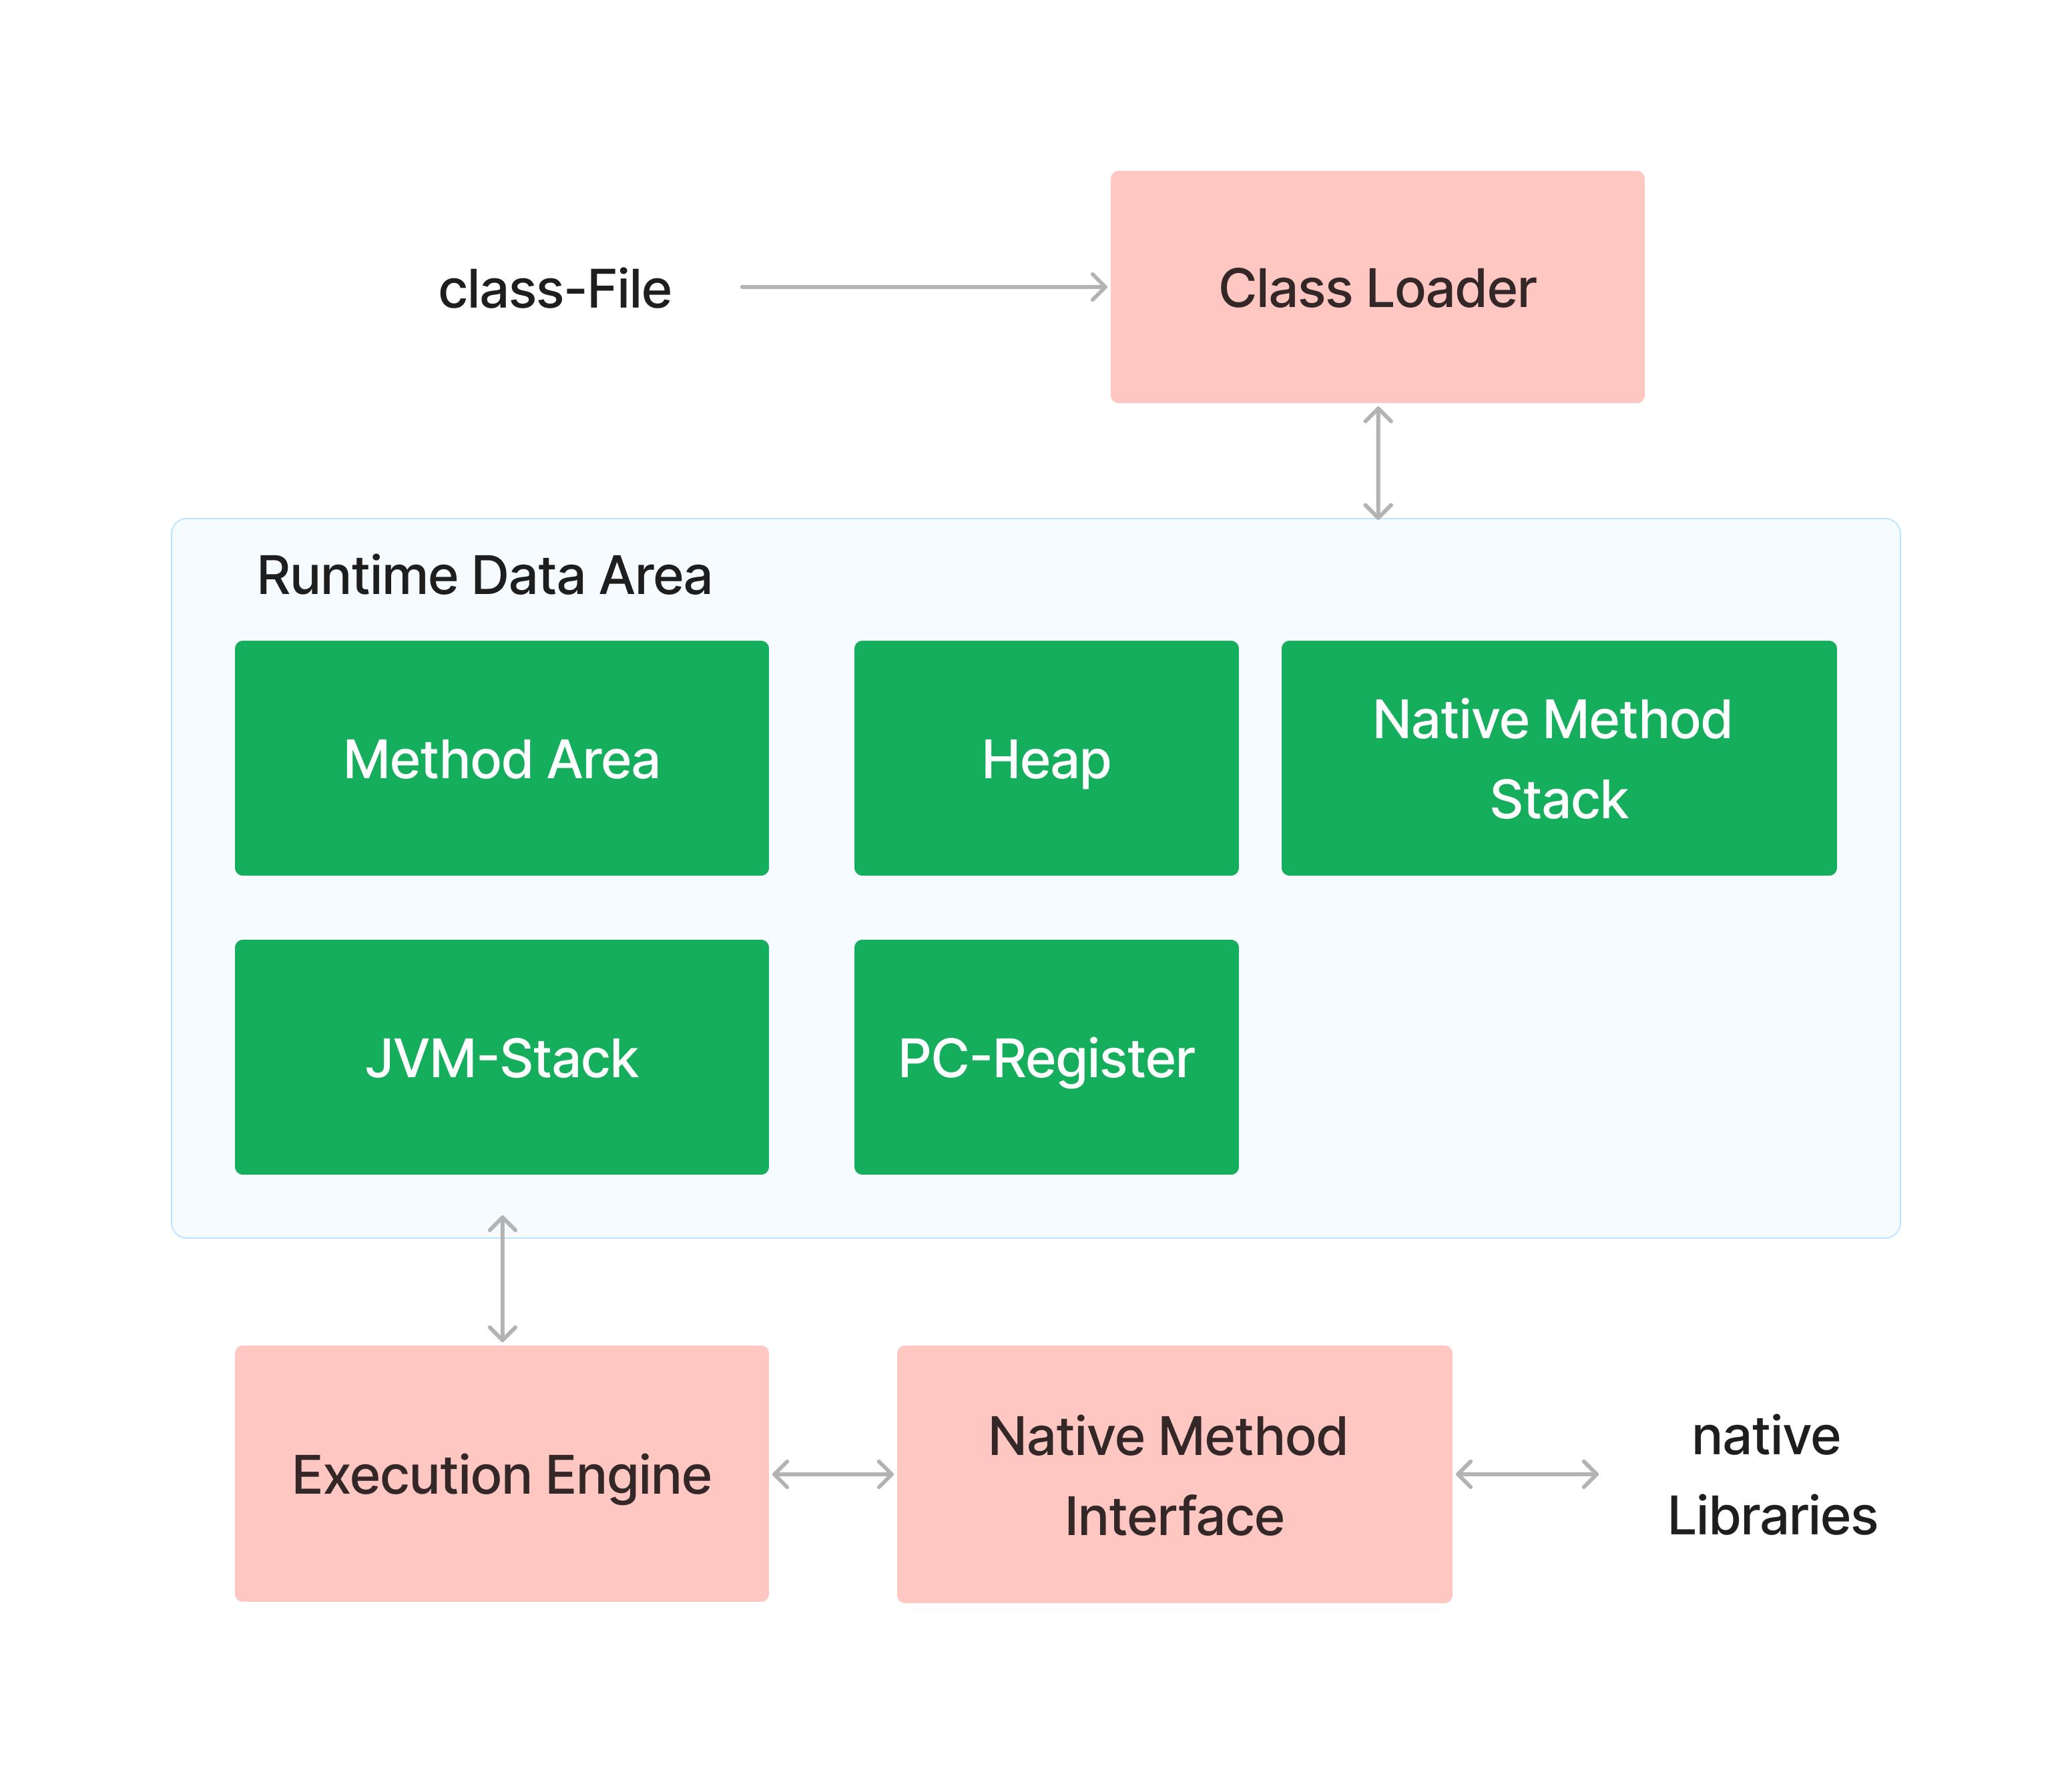
\includegraphics[width=\textwidth]{JVM_Architecture.png}
    \caption{Architecture of the JVM.}
    \label{fig:JVMArchitecture}
\end{figure}

\subsection{\texttt{class} File Format}

A \texttt{class} file contains the necessary information that is needed to execute a program on the JVM. One \texttt{class} file contains the definition of either a single class, interface or module. A \texttt{class} file is structured as follows: 

\begin{itemize}
    \item Magic Number
    \item Version Info
    \item Constant Pool
    \item Access Flags
    \item This Class
    \item Super Class
    \item Interfaces
    \item Fields
    \item Methods
    \item Attributes
\end{itemize}

At the beginning of the \texttt{class} file is the magic number. It is responsible for identifying a \texttt{class} file. The magic number is the same for every \texttt{class} file. Next is the version of the \texttt{class} file format. The JVM uses the version to determine if the \texttt{class} file is compatible with it.

The \textit{constant pool} acts as a storage for all constants and symbolic references contained in the file. For example the reference to a method or a string literal. An entry in the constant pool consists of a tag which specifies one of 17 constant types, followed by information describing the constant. Depending on the type, the length of the constant may change. A string literal for example would require more memory than an integer. 

The \textit{access flag} entry is a flag mask that defines the permissions and properties of the class or interface. Possible flags include for example, whether the class is \texttt{public, final, abstract} or not. 

The \textit{this class} entry contains the name of the current class in the form of an index to an entry in the constant pool. Analogous the \textit{super class} entry defines the name of the superclass of this class. In case that the class does not inherit from a superclass, the index is zero. The following section lists all implemented interfaces, again as a list of indexes in the constant pool. 

In the \textit{fields} section all member fields of the class are listed. Each field description consists of four elements: Access flags, similar to the class level access flags, e.g., \texttt{public, private}. An index to the name of the field in the constant pool. An index to the descriptor (type specification) of the field in the constant pool. Finally, the entry can have optional attributes associated with it, e.g., the constant value (for static fields). An entry in the \textit{methods} section contains the same values, only the descriptor is used to describe the method signature (parameter and return type).

Finally, in the \textit{attributes} section, additional metadata of the class is stored. Most importantly, this section contains the bytecode for each method of the class. Other information includes for example, a list of exceptions thrown by each method, the name of the source file or a mapping from bytecode instructions to source code line numbers.

\subsection{Class Loader}

The class loader takes care of loading bytecode into the JVM memory. There are three tiers of class loaders:

\begin{itemize}
    \item \textbf{Bootstrap}: Loads JDK internal classes and core libraries. Implemented in native code and not accessible by an application. 
    \item \textbf{Extension}: Loads extensions of the standard Java classes from the JDK extensions directory. 
    \item \textbf{Application}: Loads all application level classes. These are located via the classpath. Classes can be put on the classpath by using an environment variable or command line option. 
\end{itemize}

The class loaders are organized in a parent-child hierarchy. The Bootstrap class loader is the parent of the Extension class loader, which itself is the parent of the Application class loader. When a request is made to load a \texttt{class} file, the class loader first delegates the request to its parent class loader. Only if the parent class loader cannot locate the class the current class loader will attempt to load it. This process is performed so that no two class loaders attempt to load the same class. The loading process is separated into three stages. Loading, linking and initialization.

In the loading stage the bytecode is loaded into the JVM. The bytecode can be loaded from a file, the network or another source. The bytecode is loaded into the JVM as a \texttt{Class} object.

In the second stage linking is performed. This stage is separated into the three substages verification, preparation and resolution. Verification is performed to ensure that the loaded bytecode adheres to the JVM's rules. Rules include such as requiring that a return instruction must match its method's return type, or that a \texttt{throw} instruction must only throw values that are instances or subclasses of \texttt{Throwable}. Verification is performed because the JVM must guarantee that only correct \texttt{class} files are executed and no exploitation through malicious bytecode is taking place. The second substage preparation creates the static fields of a class or interface and allocates the memory needed for them. The static fields further are assigned their respective default values. Explicit initializers are executed during initialization, during preparation no bytecode is executed. Resolution then resolves all symbolic references inside the class. Symbolic references are used for example when referencing another class or interface. For each symbolic reference resolution determines a concrete value. 

If linking has been successful the class or interface is initialized. Explicit initializer of static fields are executed as are static initializer blocks of the class or interface.

\subsection{Runtime Data Areas}

The runtime data areas of the JVM are regions of memory used during the execution of a program. Each memory area serves a specific use case. Some memory areas are specific to a thread. They get created when a thread is created and cleaned up on thread termination. Others are alive for the entire duration of the JVM's runtime.  

\subsubsection{PC Register}

The \texttt{program counter} or PC register is the memory area which contains the bytecode instruction that is currently being executed. Each thread inside the JVM has its own PC register. In the case that a native method is executed, the PC register's value is undefined.

\subsubsection{JVM Stacks}

A JVM Stack is a thread-specific memory area that is created in tandem with the thread. A stack in the JVM is similar to a stack in languages such as C. An instance of a stack stores \textit{frames} for method-calls. On method invocation a new frame is created. Conversely, when the method invocation is finished, the frame is destroyed. 

A frame contains information related to a single method invocation. This includes the following:

\begin{itemize}
    \item Local variables and method parameters
    \item Operand stack
    \item Reference to constant pool of the method's class
    \item Return address 
\end{itemize}

The operand stack is used for intermediate calculations and storing results from other method invocations. The reference to the constant pool is needed to resolve the targets for method calls and field accesses. The return address stores the address of the calling method. Once the method invocation has completed control will be returned to this address.

\subsubsection{Heap}

In the \textit{heap} all object instances and arrays are stored. The heap is shared across all threads and is created on JVM startup. Contrary to programming languages like C, it is not possible in the JVM to manually reclaim/free the memory allocated by an object or array. Instead, the JVM utilizes an automatic storage management system known as a \textit{garbage collector}. The garbage collector automatically reclaims memory from objects and arrays that are no longer referenced by any other object or variable in the program. The JVM specification does not require a specific garbage collector algorithm, rather the implementer can choose which algorithm to use or also allow the user to select the algorithm. While the garbage collector automatically reclaims memory, it is also possible to manually request a cleanup through an API. There is however no requirement for the garbage collector to honor this request, so it may be ignored. 

\subsubsection{Method Area}

The method area is a section of the memory that is available to all threads inside the JVM and is created on JVM startup. It stores metadata of the classes loaded into the JVM. This includes the runtime constant pool, field and method data and the bytecode for methods and constructors.

\subsubsection{Native Method Stacks}

Similar to JVM stacks \textit{native method} stacks are associated with a method invocation and store information relevant to that invocation. However, in this case the invoked method is executed natively on the host system. Instead of bytecode, native code, written in e.g. C, is executed. The native method stack serves as an interface between the native code and the bytecode inside the JVM.  
  
\subsection{Execution Engine}

The JVM's execution engine is responsible for executing the bytecode contained in the loaded \texttt{class} files. It takes bytecode instructions and transforms them into something the host system can execute. This may be through interpretation or just-in-time (JIT) compilation. The JVM specification does not specify how the bytecode is executed on the host system. Therefore, in this section the execution engine \textit{HotSpot} of the JVM reference implementation \textcite{OpenJDKHotspotRuntime} is explained.

The HotSpot execution engine consists of two main parts: The interpreter and the JIT-Compiler. For memory management the execution engine is supported by the garbage collector, that automatically reclaims memory from unused objects and arrays. The java native interface (JNI) enables the JVM to call and execute code and libraries written in other languages like C or C\verb|++|.

\subsubsection{Interpreter}

The interpreter reads bytecode instructions sequentially and translates them to target code the host system can execute. This allows the JVM to start executing bytecode right away, without having to wait for any JIT compilation to be performed. In comparison, .NETs' Common Language Runtime (CLR) performs a JIT compilation of a methods' code as soon as it is first invoked\parencite{MicrosoftCILToNative}. 

HotSpot uses a template-based interpreter. On JVM startup HotSpot creates an interpreter based on the data in the so called \texttt{TemplateTable}. The \texttt{TemplateTable} contains information on the assembly code corresponding to each bytecode instruction. A template in this case is a description of a bytecode. The generated templates are specific to the host operating system and architecture. The interpreter fetches the template corresponding to the current bytecode instruction and executes it. The template is fetched by using an accessor function provided by the \texttt{TemplateTable}. This approach leads to higher performance than using a switch-statement, which may have to compare the current instruction with all cases to find the correct code to execute. A downside of this approach is the need for extra platform and operating system specific code needed for the dynamic code generation. Some operations, like a lookup in the constant pool, are still performed via the JVM runtime, since they are too complicated to be implemented in assembly code directly. 

Initially, all code on the JVM is interpreted. The runtime performs adaptive optimization by monitoring the code execution for methods that are executed often, so-called \textit{hotspots}. For those hotspots the runtime performs optimization. Specifically a method detected as a hotspot will be just-in-time compiled, so that it can be natively executed on the host system. 

\subsubsection{Just-In-Time Compilation (JIT)}

To increase performance, the JVM runtime employs just-in-time (JIT) compilation. Contrary to ahead-of-time compilation, which translates the code before the execution, JIT compilation translates the code during the execution of the program. Because the compilation is performed while the program is executing, considerations need to be made about the performance implication of the compilation. Therefore, the JVM uses a two stage tiered compilation: The C1 or \textit{client} compiler and the C2 or \textit{server} compiler.

%https://cr.openjdk.org/~vlivanov/talks/2015_JIT_Overview.pdf

Through profiling the JVM runtime identifies hotspots, also referred to as \textit{hot methods}. These are methods that are executed often. Methods that are only called rarely are referred to as \textit{cold methods}. The JIT compiler focuses only on hot methods for multiple reasons: Compiling bytecode to native code takes up processor time that cannot be used for the actual execution of the program. Furthermore, the compiled code needs to be stored in memory and thus completely compiling bigger programs to native code make take up a significant amount of memory. Only compiling hot methods strikes a balance between performance and memory consumption. Also, empirically programs spend most of their execution time on a small amount of the entire codebase. 

Once a method has been identified for compilation, the first JIT compiler C1 compiles the method to native code. The C1 compiler prioritizes compilation speed and therefore only performs basic optimizations. After compilation the methods' body is replaced by the compiled code, leading to the method being executed natively and no longer interpreted. During compilation code used for profiling is also added. The profiling information is used for the second stage of the JIT compilation. 

When a method that was compiled with C1 passes an execution threshold, the C2 compiler will compile the method again. This time the focus is on performing aggressive optimizations for maximum performance, which consumes more times than the first compilation. The C2 compiler uses the information gained through profiling to perform optimizations that lead to the best performance. This may include optimization techniques such as loop unrolling or inlining. The C2 compiler does not add any code for profiling which further improves performance. In some cases the assumptions that the C2 compiler made based on the profiling data can turn out to be wrong, which in turn can lead to the method being returned to the C1 compilation level.

\subsubsection{Java Native Interface (JNI)}


\begin{JavaCode}[float,numbers=none,caption=Declaration of a native method in Java., label=lst:JNINativeMethod]
    public class Example {
        public native void nativeMethod();
    }
\end{JavaCode}


The Java Native Interface (JNI) is an API that enables the code executed inside the JVM to interoperate with applications and libraries that are written in other languages. This API is necessary because there are cases when the entirety of the application cannot be implemented inside the JVM. For example there might be libraries only available in C/C++, but not for the JVM. The JNI then allows calling those libraries from within the JVM. Listing \ref{lst:JNINativeMethod} shows the declaration of a native method in Java. The \texttt{native} keyword signalizes to the JVM that the implementation of the method will be provided in native code.


The JNI makes it possible to create, inspect and update JVM objects. For that the JNI provides a type mapping between the JVM types and native equivalents. Further, methods located inside the JVM can be called or exceptions thrown from within native code.

Using the JNI inside an application however limits the number of systems it can be executed on. The native part of the application needs to be compiled for every architecture and operating system the application is intended to run on. Native methods manually manage the memory they have allocated and therefore programming errors can lead to memory leaks within the application.  

\section{Bytecode}

Bytecode is the instruction set of the JVM. It serves as an intermediate language between high level languages such as Java or Kotlin, and low level languages such as assembly which can be natively executed on a CPU. High level languages only need to target bytecode to be cross-platform. As long as a JVM implementation is present for a given architecture and operating system, the bytecode can be executed without needing to be compiled again. 

\subsection{Structure}

In terms of code execution JVM is organized as a stack machine with registers. Each method being executed is structured as a frame containing an operand stack and local variables, which can be seen as registers. The operand stack and number of variables inside a frame are each able to contain up to 65535 entries.

A bytecode instruction is structured as a one byte long opcode followed by zero or more one byte long operands. The maximum possible number of opcodes is therefore 256. Most of them are in use, while some are reserved for internal and future use. Each instruction has a mnemonic associated with it. Instructions that can operate on multiple types are prefixed by the concrete type they are operating on. For example the instruction for adding together two integers is known by the mnemonic \texttt{iadd}. The following types are supported in bytecode:

\begin{itemize}
    \item \texttt{boolean}
    \item \texttt{byte}
    \item \texttt{char}
    \item \texttt{short}
    \item \texttt{int}
    \item \texttt{float}
    \item \texttt{reference}
    \item \texttt{returnAddress}
    \item \texttt{long}
    \item \texttt{double}
\end{itemize}

Most instructions for the types \texttt{byte}, \texttt{char} and \texttt{short} and all for \texttt{boolean} are internally converted to \texttt{int}, therefore in these cases the \texttt{int} based instructions are used instead.

The \texttt{reference} type is analogous to pointer types in languages like C. It is type-safe and managed by the JVM. The JVM also keeps track of the references for garbage collection purposes. If there are no references anymore pointing to an object, the garbage collector can reclaim the memory it occupied. The \texttt{returnAddress} type represents pointers to opcodes of JVM instructions. This type is only used internally and is not accessible otherwise.


\subsection{Categories of Instructions}

The instructions in the bytecode instruction set can be categorized depending on their functionality. Instructions from each category work together to perform more complex actions. 

\subsubsection{Load and Store Instructions}

Load and store instructions allow the loading of values onto the operand stack and storing values from it into variables. These instructions function within the frame of a method. Load instructions like \texttt{iload} or \texttt{aload} load an integer or array respectively onto the operand stack. To load a constant onto the operand stack instructions like \texttt{bipush} and \texttt{ldc} can be used. \texttt{ldc} loads a constant from the constant pool of the class while \texttt{bipush} takes one operand (the constant value), that is loaded onto the operand stack. When a value from the operand stack is to be stored into a variable instructions like \texttt{istore} or \texttt{astore} are available. 

\subsubsection{Arithmetic Instructions}

Arithmetic instructions perform calculations using the values on the operand stack. The result of the calculation is then put on the operand stack. There are separate instructions for integer and floating point calculations, e.g. \texttt{iadd} and \texttt{fadd} for integer and floating point additions respectively. In the case of an over or underflow no exception is thrown. The bytecode instruction set further includes instructions for bitwise logical operations like AND (\texttt{iand}). 

\subsubsection{Type Conversion Instructions}

Type conversion instructions make it possible to change the type of a numeric value. They can be used to perform an explicit conversion. The JVM supports widening conversions (e.g. from \texttt{int} to \texttt{long}; \texttt{i2l}) and narrowing conversions (e.g. from \texttt{float} to \texttt{int}; \texttt{f2i}). For some conversions there may be a loss of information. Widening conversions like from \texttt{int} to \texttt{float} can lose some of the least significant bits of the source value. 

\subsubsection{Object related Instructions}

The bytecode instruction set contains separate instructions for class instances and arrays, even though they are both considered as objects by the JVM. To create a class instance the instruction \texttt{new} is used, while for an array \texttt{newarray} is used. To access class fields the \texttt{getfield} instruction can be used for instance variables and \texttt{getstatic} for class variables. When loading an entry from an array there is a separate instruction for each type, e.g. \texttt{iaload} for loading an integer from an array. For storing a value inside a class instance or array analogous instructions are available. 

\subsubsection{Operand Stack Management Instructions}

In some cases it is beneficial to perform manipulations on the operand stack directly. For example to implement peephole optimization, it is necessary to duplicate a value on the operand stack as an alternative to loading a variable two times\parencite{mckeeman1965peephole}. The instruction for that is \texttt{dup}. The instruction set further provides instructions like \texttt{pop} or \texttt{swap}. 

\subsection{Sample program}